%% bare_jrnl_compsoc.tex
%% V1.4a
%% 2014/09/17
%% by Michael Shell
%% See:
%% http://www.michaelshell.org/
%% for current contact information.
%%
%% This is a skeleton file demonstrating the use of IEEEtran.cls
%% (requires IEEEtran.cls version 1.8a or later) with an IEEE
%% Computer Society journal paper.
%%
%% Support sites:
%% http://www.michaelshell.org/tex/ieeetran/
%% http://www.ctan.org/tex-archive/macros/latex/contrib/IEEEtran/
%% and
%% http://www.ieee.org/

%%*************************************************************************
%% Legal Notice:
%% This code is offered as-is without any warranty either expressed or
%% implied; without even the implied warranty of MERCHANTABILITY or
%% FITNESS FOR A PARTICULAR PURPOSE! 
%% User assumes all risk.
%% In no event shall IEEE or any contributor to this code be liable for
%% any damages or losses, including, but not limited to, incidental,
%% consequential, or any other damages, resulting from the use or misuse
%% of any information contained here.
%%
%% All comments are the opinions of their respective authors and are not
%% necessarily endorsed by the IEEE.
%%
%% This work is distributed under the LaTeX Project Public License (LPPL)
%% ( http://www.latex-project.org/ ) version 1.3, and may be freely used,
%% distributed and modified. A copy of the LPPL, version 1.3, is included
%% in the base LaTeX documentation of all distributions of LaTeX released
%% 2003/12/01 or later.
%% Retain all contribution notices and credits.
%% ** Modified files should be clearly indicated as such, including  **
%% ** renaming them and changing author support contact information. **
%%
%% File list of work: IEEEtran.cls, IEEEtran_HOWTO.pdf, bare_adv.tex,
%%                    bare_conf.tex, bare_jrnl.tex, bare_conf_compsoc.tex,
%%                    bare_jrnl_compsoc.tex, bare_jrnl_transmag.tex
%%*************************************************************************


% *** Authors should verify (and, if needed, correct) their LaTeX system  ***
% *** with the testflow diagnostic prior to trusting their LaTeX platform ***
% *** with production work. IEEE's font choices and paper sizes can       ***
% *** trigger bugs that do not appear when using other class files.       ***                          ***
% The testflow support page is at:
% http://www.michaelshell.org/tex/testflow/


\documentclass[10pt,conference,onecolumn,compsoc]{IEEEtran}


\usepackage{hyperref}
\usepackage{enumitem}
\setlist[itemize]{leftmargin=3 cm}
\setlist[enumerate]{leftmargin=3cm}



% *** CITATION PACKAGES ***
%
\ifCLASSOPTIONcompsoc
  % IEEE Computer Society needs nocompress option
  % requires cite.sty v4.0 or later (November 2003)
  \usepackage[nocompress]{cite}
\else
  % normal IEEE
  \usepackage{cite}
\fi
% cite.sty was written by Donald Arseneau
% V1.6 and later of IEEEtran pre-defines the format of the cite.sty package
% \cite{} output to follow that of IEEE. Loading the cite package will
% result in citation numbers being automatically sorted and properly
% "compressed/ranged". e.g., [1], [9], [2], [7], [5], [6] without using
% cite.sty will become [1], [2], [5]--[7], [9] using cite.sty. cite.sty's
% \cite will automatically add leading space, if needed. Use cite.sty's
% noadjust option (cite.sty V3.8 and later) if you want to turn this off
% such as if a citation ever needs to be enclosed in parenthesis.
% cite.sty is already installed on most LaTeX systems. Be sure and use
% version 5.0 (2009-03-20) and later if using hyperref.sty.
% The latest version can be obtained at:
% http://www.ctan.org/tex-archive/macros/latex/contrib/cite/
% The documentation is contained in the cite.sty file itself.



% *** GRAPHICS RELATED PACKAGES ***
%
\ifCLASSINFOpdf
   \usepackage[pdftex]{graphicx}
 
\else
 
\fi
% graphicx was written by David Carlisle and Sebastian Rahtz. It is
% required if you want graphics, photos, etc. graphicx.sty is already
% installed on most LaTeX systems. The latest version and documentation
% can be obtained at: 
% http://www.ctan.org/tex-archive/macros/latex/required/graphics/
% Another good source of documentation is "Using Imported Graphics in
% LaTeX2e" by Keith Reckdahl which can be found at:
% http://www.ctan.org/tex-archive/info/epslatex/
%
% latex, and pdflatex in dvi mode, support graphics in encapsulated
% postscript (.eps) format. pdflatex in pdf mode supports graphics
% in .pdf, .jpeg, .png and .mps (metapost) formats. Users should ensure
% that all non-photo figures use a vector format (.eps, .pdf, .mps) and
% not a bitmapped formats (.jpeg, .png). IEEE frowns on bitmapped formats
% which can result in "jaggedy"/blurry rendering of lines and letters as
% well as large increases in file sizes.
%
% You can find documentation about the pdfTeX application at:
% http://www.tug.org/applications/pdftex









% *** PDF, URL AND HYPERLINK PACKAGES ***
%
\usepackage{url}
% url.sty was written by Donald Arseneau. It provides better support for
% handling and breaking URLs. url.sty is already installed on most LaTeX
% systems. The latest version and documentation can be obtained at:
% http://www.ctan.org/tex-archive/macros/latex/contrib/url/
% Basically, \url{my_url_here}.

\usepackage{float}


\begin{document}

\title{RPG Character Creator}
%
%

% received ..."  text while in non-compsoc journals this is reversed. Sigh.

\author{Ethan Buchanan and Steven Garcia-Alamilla \\% <-this % stops a space
}

\IEEEtitleabstractindextext{%
\begin{abstract}
The RPG Character Creator is a tool that lets users create their own characters for RPG games, from Tabletop RPG enthusiasts to casual gamers. The project is close to a finished state and allows the user create a character from a predefined set of classes, races, backgrounds, and skills. The program allows you to save your characters so you can come back and look at your created character. It also allows you to edit and delete previously created characters.
\end{abstract}

}


% make the title area
\maketitle



\IEEEdisplaynontitleabstractindextext

\IEEEpeerreviewmaketitle



\section{Introduction}



Character creation is a very important part of any RPG (Role Playing Game) experience. The RPG Character Creator is designed to provide an easy way to plan out future RPG journeys, whether you are an experienced RPG veteran or new to the RPG genre, the RPG Character Creator will provide a fun and engaging way to customize certain aspects of your character.While it is not necessary to plan out your character in advance, doing so allows stronger, more focused characters that can make your experience playing through the game better. While we can't provide a RPG character creator that covers every RPG system, we do hope our more generalized system allows the user to create a character that covers many different games. The tool can also be used not just for tabletop games, but can also be used to design a character for video games and even can be used for planning characters for something such as a novel.
% needed in second column of first page if using \IEEEpubid
%\IEEEpubidadjcol

\subsection{Background}
If you are unfamiliar with the RPG (Role-Playing Game) genre, there are a few things you should know. Firstly, RPGs allow you to play the role of a fictional character in a narrative-driven story. You are then given the ability to create and customize you character choosing who and what you want to play as. Some different attributes that you might be able to customize would include:
\begin{itemize}
\item Name, Biography, Age, Gender and Birthday
\item Appearance of your character through AI generated portraits or import your own image
\item Predefined Classes
\item Predefined Races
\item Predefined Backgrounds
\item Choose your character's stats and skills
\end{itemize}

\subsection{Impacts}
While this project might not be impactful to everyone,we hope that the RPG Character Creator will have a major impact with people who enjoy playing RPG games. It would allow for users to plan out their character for their next RPG journey, which can enhance their overall experience.

\subsection{Challenges}
A few challenges that we anticipate through the course of this project include:
\begin{itemize} 
\item Limitations of WPF
\item Creating a GUI that makes it easy for the user to navigate through.
\item Being able to finish the project on time.
\end{itemize}

A way we would overcome these challenges is by following the stages in the waterfall software development life cycle (SDLC). The SDLC makes sure that as we progress through the different phases of this project we keep in mind what has to be accomplished in order to move forward to the next stage.

As we wrap of development of the program outside of stretch goals, some challenges that came up when developing the application was updating the UI dynamically, getting finished in time, and not letting the project get too overwhelming. As the first demo day approached, we had little of the project done. We got a reasonable amount done for it, but before that deadline was set, we had problems getting started. There was always that question of "Where do we even start?", but we did some research of WPF applications and that allowed us to get a somewhat working UI out for the demo. A lot of this project did not have a lot of hard parts but many different small parts that required some work. We should of sat down and came up with a list of what races, classes, and backgrounds and had all of the information required for each done before it came time to implement them, but we ended up just winging it.


\section{Scope}
The completion of the project would mean that the user can create multiple RPG characters by customizing the character's Name, Portrait, Class, Race, Background, Stats, Skills and alignment.
The RPG Character Creator would show the list of characters that have been created allowing for the creation/deletion of characters and even modifying characters after they have been created.
A few stretch goals we have include:
\begin{itemize} 
\item Different rule sets for different types of RPGs (example: Fallout/ DnD 5e)
\item Allow for the user to toggle a DM mode which allows them to add custom skills, abilities, races, and  classes to the character creator allowing for more customization of characters.
\end{itemize}
The implementation is done for everything outside of the designated stretch goals. There is still areas of improvement that need to be made for the base program, the main program mostly works bug-free.

\subsection{Requirements}
We want to make sure that our project meets the user's needs, so we looked at similar RPG character creator websites and looked at a variety of different video game character creators to understand what is required to create a fulfilling character creator that does not make the user want for more customization. We found that users prefer something that's easy to use, responsive, and gives the user many different options. Based on what we found users preferred, we created these requirements for our application.

\subsubsection{Functional}
\begin{itemize}
\item The user should be able to create a new character.
\item The user should be able to customize their character's stats, skills, abilities, choose from a large list of classes, choose from a wide variety of different races, and their character's background
\item The user should be able to manage their characters by viewing, editing, and deleting them
\end{itemize}

\subsubsection{Non-Functional}
\begin{itemize}
\item The application should be easy to use allowing the user to easily navigate through the GUI making it a more pleasant experience.
\item Users will be able to use RPG Character creator without it feeling choppy or unresponsive.
\end{itemize}

\subsection{Use Cases}
\begin{table}
\centering
\begin{tabular}{|c|c|c|c|c|}
\hline
Use Case ID & Use Case Name & Primary Actor & Complexity & Priority \\
\hline \hline
1 &  Create New Character & User & Med & 1\\
\hline
2 & Fill out Character Bio/Information & User & Low & 2\\
\hline
3 & Choose Character Portrait & User & Hard & 3\\
\hline
4 & Choose Character Class & User & Low & 2\\
\hline
5 & Choose Character Race & User & Low & 2\\
\hline
6 & Choose Character Background & User & Med & 2\\
\hline
7 & Choose Character Skills & User & Med & 3\\
\hline
8 & Choose Character Abilities & User & Med & 3\\
\hline
9 & Choose Character Alignment & User & Low & 2\\
\hline
10 & Finish Character on Overview Screen & User & Med & 1\\
\hline
11 & Edit Character and Delete Character & User & Med & 4\\



\end{tabular}
\caption{RPG Character Creator Use Case Table}
\label{tab:useCaseIndex}
\end{table}


\begin{itemize}
\item[Use Case Number:] 1
\item[Use Case Name:] Create New Character
\item[Description:] The user starts the process for creating a new character.They will click on the “Create New Character” button this will take User to the character creator menu starting with the character information screen. 
\end{itemize}

Basic flow for the process:

\begin{enumerate}
\item User navigates to the “Create new Character” button
\item User left-clicks on the button.
\item User is taken the character creation screen.
\item[Termination Outcome:] The user is now in the process of creating a new character. The user begins on the character info screen.
\end{enumerate}

\begin{figure}[ht!]
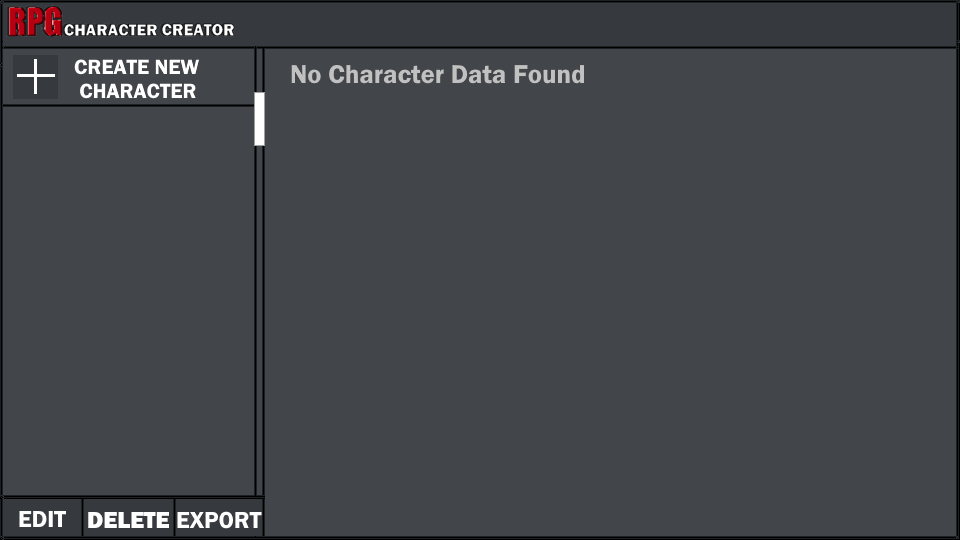
\includegraphics[height=180px, width=320px]{CSCI 352 Interface Mockups/Interface Mockup 0.5.png}
\caption{Use Case 1: What a user would see with no characters created.}
\centering
\label{mockup0.5}
\end{figure}

\begin{itemize}
\item[Use Case Number:] 2
\item[Use Case Name:] Fill Out Character Bio/Information
\item[Description:] The user is now underway with creating their character. They have been taken to the first tab of character creation: the character information screen where they will fill in the Character's bio and basic information like name, age, gender, etc.
\end{itemize}
Basic flow for the process:
\begin{enumerate}
\item User is now on Character Bio screen
\item User can fill in each field for character info.
\item User can fill in character's back story.
\item[Termination Outcome:] To leave this screen the user can click on the tabs at the top of the screen to go to a different category of character creation.
\end{enumerate}

\begin{figure}[ht!]
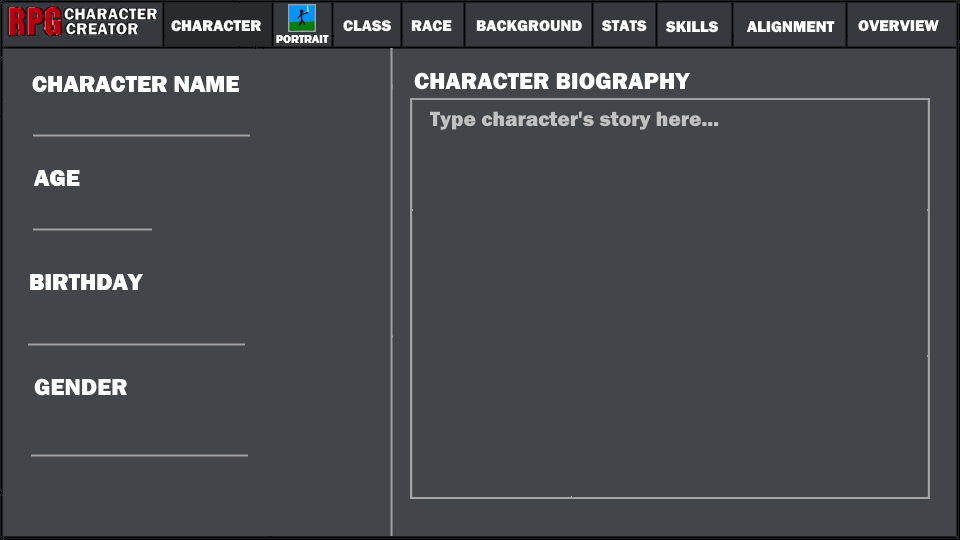
\includegraphics[height=180px, width=320px]{CSCI 352 Interface Mockups/Interface Mockup 4.png}
\caption{Use Case 2: What a user would see with no character info screen.}
\centering
\label{mockup4}
\end{figure}

\begin{itemize}
\item[Use Case Number:] 3
\item[Use Case Name:] Choose Character Portrait.
\item[Description:] Once the user has reached this screen, they can choose a portrait that will represent their character.
\end{itemize}
Basic flow for the process:
\begin{enumerate}
\item User is now on Character Portrait screen
\item User can choose from an already collected group of portraits.
\item User can import their own portrait for their character.
\item[Termination Outcome:] To leave this screen the user can click on the tabs at the top of the screen to go to a different category of character creation.
\end{enumerate}

\begin{itemize}
\item[Use Case Number:] 4
\item[Use Case Name:] Choose Character Class.
\item[Description:] Once the user has reached this screen, they can choose a class for their character.
\end{itemize}
Basic flow for the process:
\begin{enumerate}
\item User is now on Character Class screen
\item User can scroll up and down the list to see what class they want.
\item By clicking on a class it will select what class they want to be.
\item Clicking on a class also shows a description of what each class is as well as the class's primary and secondary stats, class skills, and class abilities.
\item[Termination Outcome:] To leave this screen the user can click on the tabs at the top of the screen to go to a different category of character creation.
\end{enumerate}

\begin{figure}[ht!]
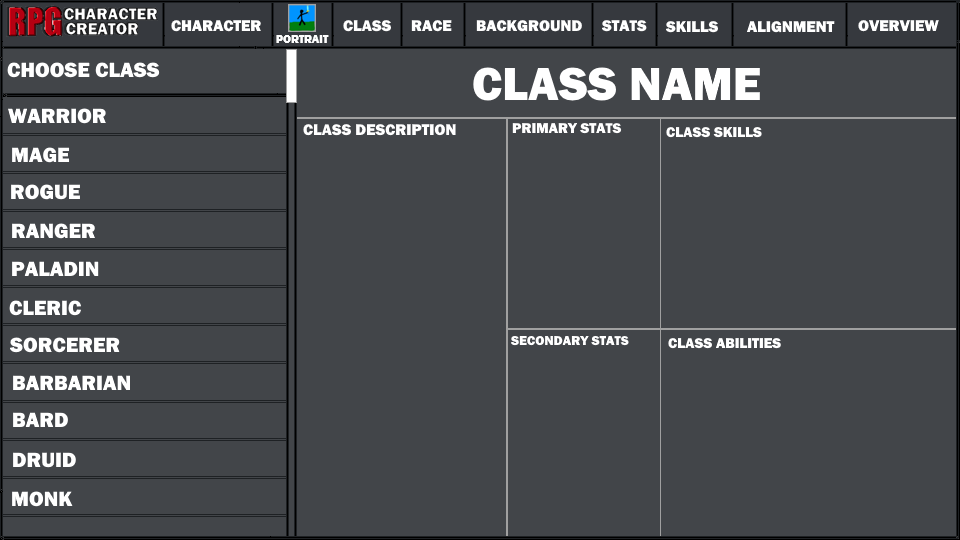
\includegraphics[height=180px, width=320px]{CSCI 352 Interface Mockups/Interface Mockup 2.png}
\caption{Use Case 4: What a user would see on the Character Class screen}
\centering
\label{mockup2}
\end{figure}

\begin{itemize}
\item[Use Case Number:] 5
\item[Use Case Name:] Choose Character Race.
\item[Description:] Once the user has reached this screen, they can choose a race for their character.
\end{itemize}
Basic flow for the process:
\begin{enumerate}
\item User is now on Character Race screen
\item User can scroll up and down the list to see what race they want.
\item By clicking on a race it will select what race they want to be.
\item Clicking on a race also shows a description of what each race is as well as the race's traits.
\item[Termination Outcome:] To leave this screen the user can click on the tabs at the top of the screen to go to a different category of character creation.
\end{enumerate}

\begin{figure}[H]
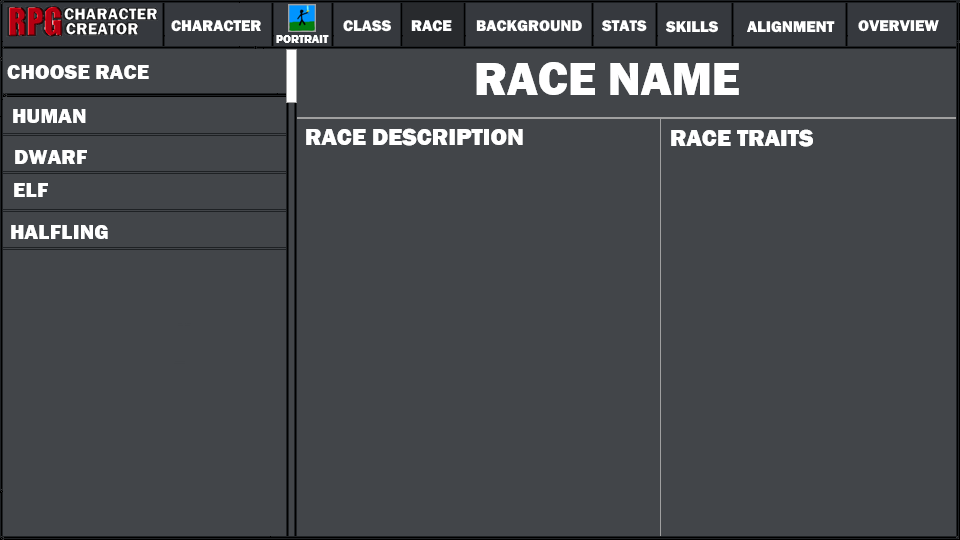
\includegraphics[height=180px, width=320px]{CSCI 352 Interface Mockups/Interface Mockup 3.png}
\caption{Use Case 5: What a user would see on the Character Race screen}
\centering
\label{mockup3}
\end{figure}

\begin{itemize}
\item[Use Case Number:] 6
\item[Use Case Name:] Choose Character Background.
\item[Description:] Once the user has reached this screen, they can choose a background for their character.
\end{itemize}
Basic flow for the process:
\begin{enumerate}
\item User is now on Character Background screen
\item User can scroll up and down the list to see what background they want.
\item By clicking on a background it will select what background they want to be.
\item Clicking on a race also shows a description of what each background is as well as what skills the background provides.
\item[Termination Outcome:] To leave this screen the user can click on the tabs at the top of the screen to go to a different category of character creation.
\end{enumerate}

\begin{itemize}
\item[Use Case Number:] 7
\item[Use Case Name:] Choose Character Skills.
\item[Description:] Once the user has reached this screen, they can choose what skills they want their character to have. There is universal skills and class specific skills.
\end{itemize}
Basic flow for the process:
\begin{enumerate}
\item User is now on Character Skills screen
\item User can scroll up and down the list to see what skills they want.
\item By clicking on a skill it will select what skills they want to add to their character, they can add multiple skills.
\item Clicking on a skill also shows a description of what each skill entails.
\item[Termination Outcome:] To leave this screen the user can click on the tabs at the top of the screen to go to a different category of character creation.
\end{enumerate}

\begin{itemize}
\item[Use Case Number:] 8
\item[Use Case Name:] Choose Character Abilities.
\item[Description:] Once the user has reached this screen, they can choose what abilities they want their character to have. There is universal abilities and class/race specific abilities.
\end{itemize}
Basic flow for the process:
\begin{enumerate}
\item User is now on Character Abilities screen
\item User can scroll up and down the list to see what abilities they want.
\item By clicking on a skill it will select what abilities they want to add to their character, they can add multiple abilities.
\item Clicking on a abilities also shows a description of what each abilities entails.
\item[Termination Outcome:] To leave this screen the user can click on the tabs at the top of the screen to go to a different category of character creation.
\end{enumerate}

\begin{itemize}
\item[Use Case Number:] 9
\item[Use Case Name:] Choose Character Alignment.
\item[Description:] Once the user has reached this screen, they can choose what abilities they want their character to have. There is universal abilities and class/race specific abilities.
\end{itemize}
Basic flow for the process:
\begin{enumerate}
\item User is now on Character Alignment screen
\item User can mouse over each alignment which will give them a description of what kind of character falls in to each alignment.
\item Clicking on a alignment choose that alignment for their character.
\item[Termination Outcome:] To leave this screen the user can click on the tabs at the top of the screen to go to a different category of character creation. At this point if the user went in order, they would go to the Overview tab.
\end{enumerate}

\begin{itemize}
\item[Use Case Number:] 10
\item[Use Case Name:] Finish Character on Overview Screen
\item[Description:] Once the user has reached this screen, they are on the final section. This screen gives an overview of what they selected and they can finally add the character to the system.
\end{itemize}
Basic flow for the process:
\begin{enumerate}
\item User is now on Character Overview screen.
\item User can now see all of what they have chosen for their character.
\item Clicking on "Finish Character Creation" will add the character to the main menu.
\item[Termination Outcome:] Once the user clicks the "Finish Character Creation" button they are taken to the main menu, exiting the character creation screen.
\end{enumerate}

\begin{figure}[H]
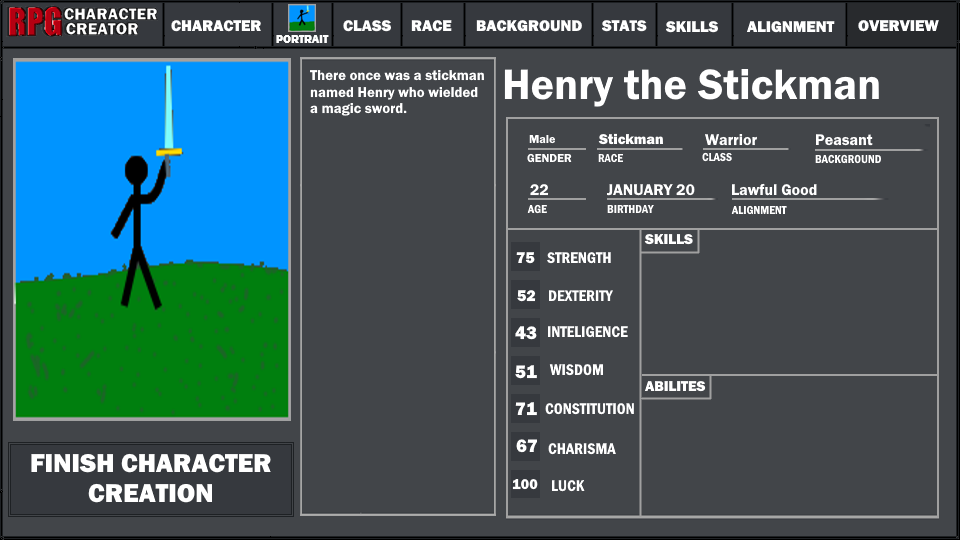
\includegraphics[height=180px, width=320px]{CSCI 352 Interface Mockups/Interface Mockup 5.png}
\caption{Use Case 10: What a user would see on the Character Overview screen}
\centering
\label{mockup5}
\end{figure}

\begin{itemize}
\item[Use Case Number:] 11
\item[Use Case Name:] Edit Character and delete character
\item[Description:] If there are characters in the system then the user can go back and edit their characters allowing them to go back through the character creation screen.
\end{itemize}
Basic flow for the process:
\begin{enumerate}
\item User is on Main Menu screen
\item User can click on character they want to select in left tab.
\item User can then navigate to bottom left of screen and press the Edit button or delete button
\item This will then take them back to the character creation menu or deletes the selected character.
\item[Termination Outcome:] Once the user has edited the character to how they want they will go back to the Overview screen and press "Finish character Creation" button again.
\end{enumerate}

\begin{figure}[ht!]
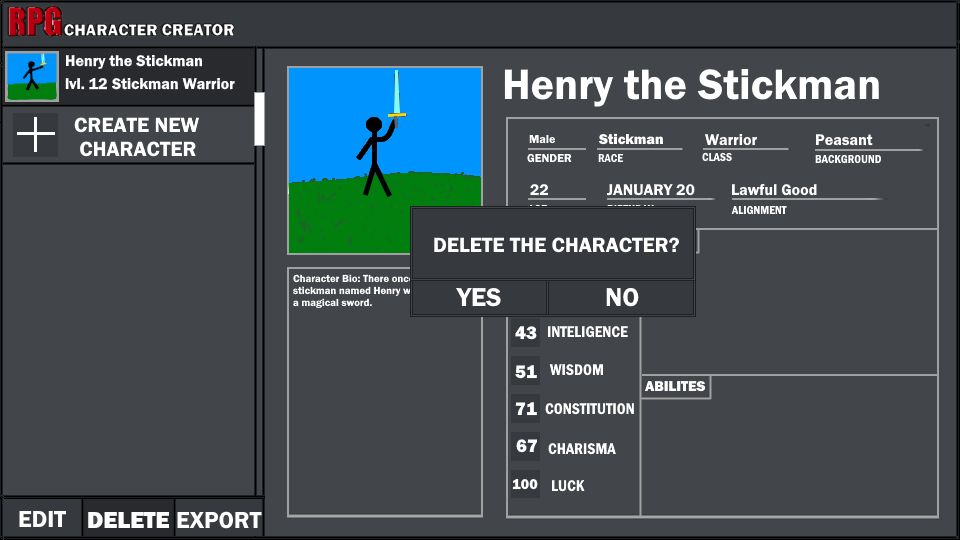
\includegraphics[height=180px, width=320px]{CSCI 352 Interface Mockups/Interface Mockup 1.5.png}
\caption{Use Case 12: What a user would see on when deleting a character}
\centering
\label{mockup}
\end{figure}

\begin{itemize}
\item[Use Case Number:] 13
\item[Use Case Name:] Export Character
\item[Description:] If there are characters in the system that the user wants to export to a file then they can.
\end{itemize}
Basic flow for the process:
\begin{enumerate}
\item User is on Main Menu screen
\item User can click on character they want to select in left tab.
\item User can then navigate to bottom left of screen and press the export button.
\item A menu showing where they want to export the character file to will show up and they choose where.
\item[Termination Outcome:] Once the user has chosen the location then, they character sheet should be saved to their computer.
\end{enumerate}

\subsection{Interface Mockups}
	Screenshots of what the final UI looks like. Once the program is started the user is met with an empty screen, with the only thing showing up is a message saying "No Character Data Found" and the create character button. If the user has started the program before then the saved characters should appear. Note, characters will only save if they have been finished, by selecting the finish character button on the Overview screen and the user exits the program through the X in the top right corner. Also, to get back to the main menu, the user needs to press on the RPG Character Creator logo.
\begin{figure}[H]
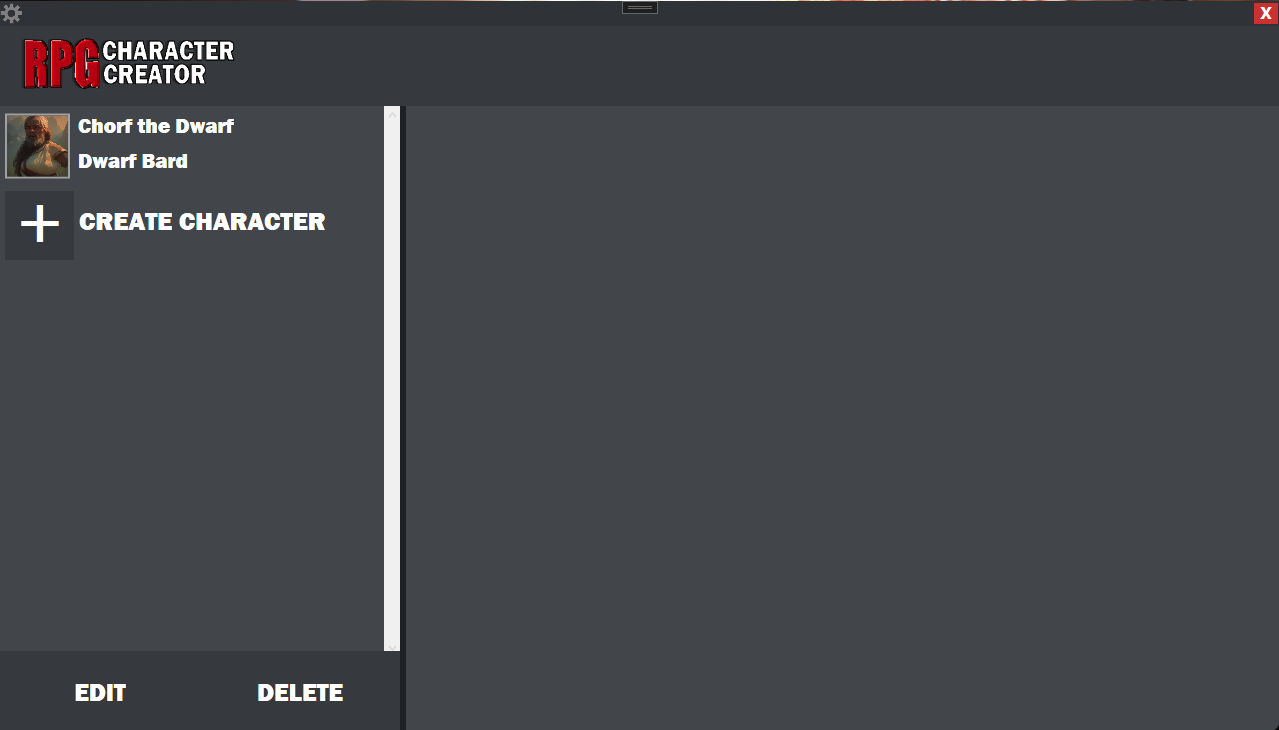
\includegraphics[height=240px, width=426px]{Finished Interface/mainScreen.png}
\caption{Main Screen, nothing selected}
\centering
\end{figure}
\begin{figure}[H]
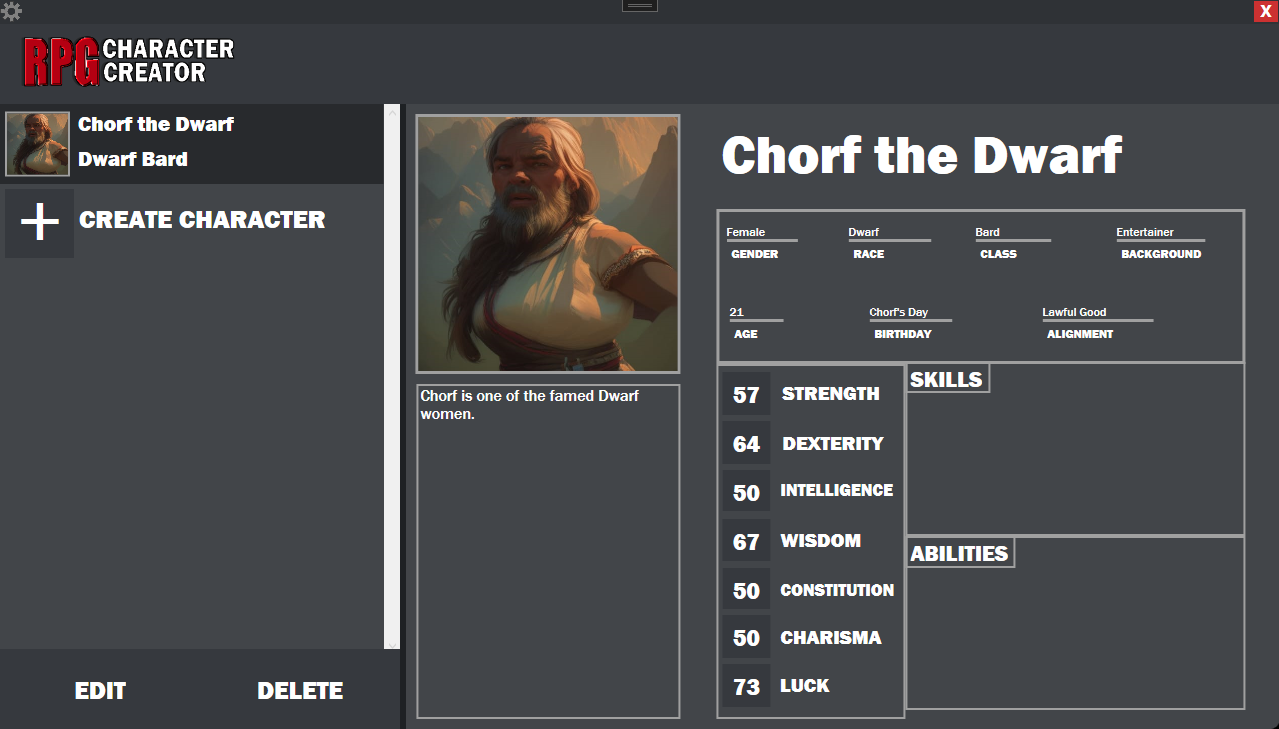
\includegraphics[height=240px, width=426px]{Finished Interface/mainScreenSelected.png}
\caption{Main Screen, character selected}
\centering
\end{figure}
The user can select their characters on this page by clicking the button. Selected characters can be edited or deleted. Pressing the edit button take the user back through character creation.
\begin{figure}[H]
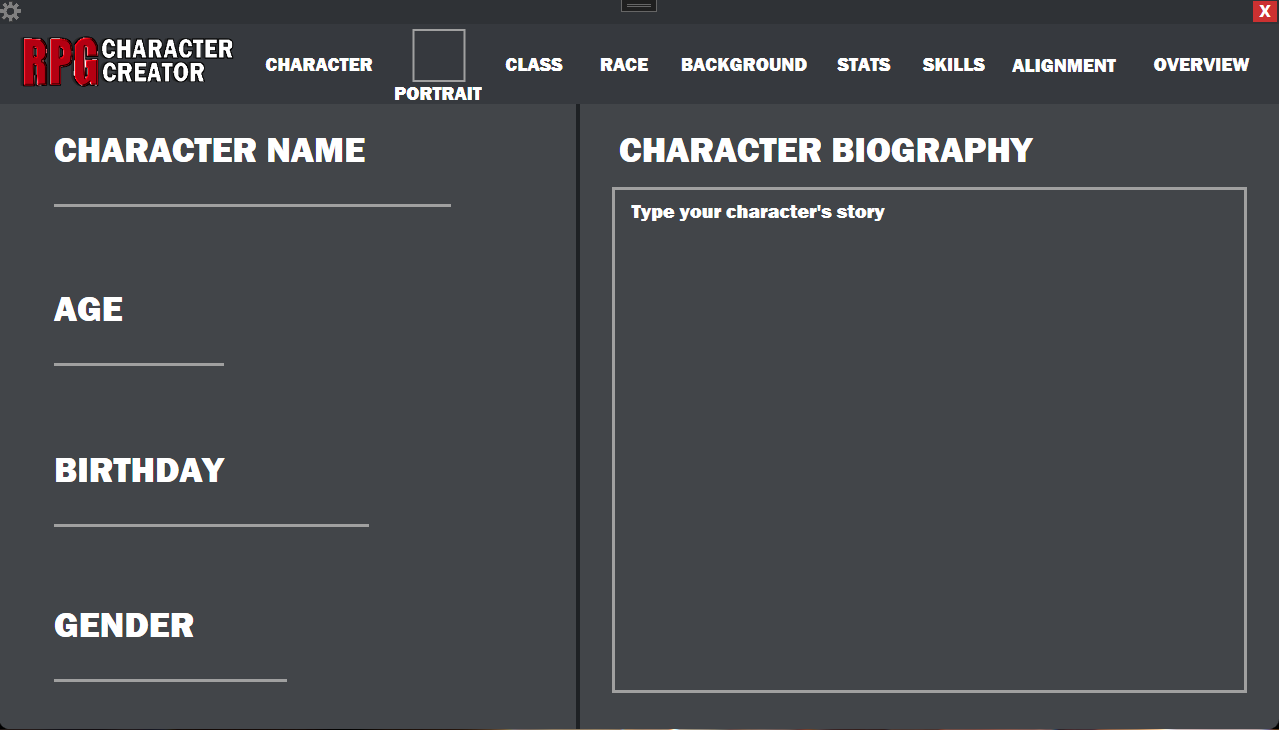
\includegraphics[height=240px, width=426px]{Finished Interface/charInfoScreen.png}
\caption{Character Bio screen}
\centering
\end{figure}
The user inputs the character info into the text boxes. To continue character creation press any of the other tabs at the top of the screen. The user can come back to the character tab later if they need to.
\begin{figure}[H]
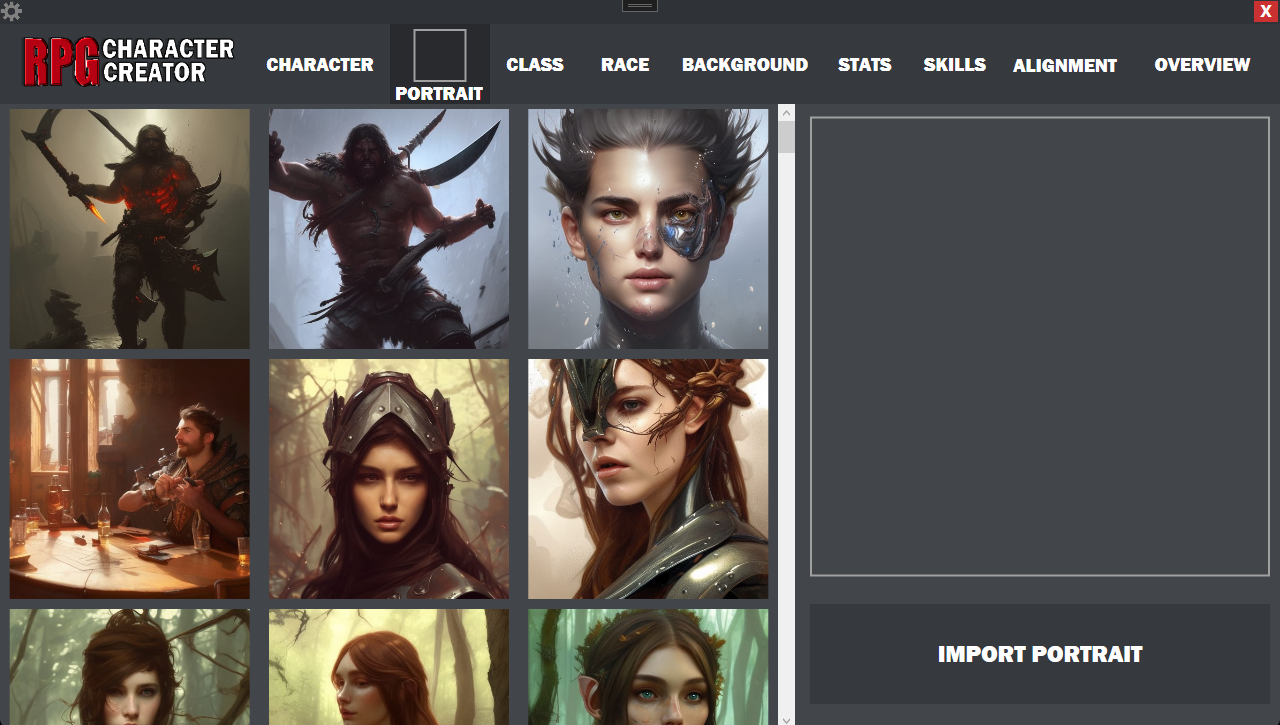
\includegraphics[height=240px, width=426px]{Finished Interface/portraitScreen.png}
\caption{Portrait Screen}
\centering
\end{figure}
The user can select a portrait from the ones provided or import their own image by pressing the import portrait button.
\begin{figure}[H]
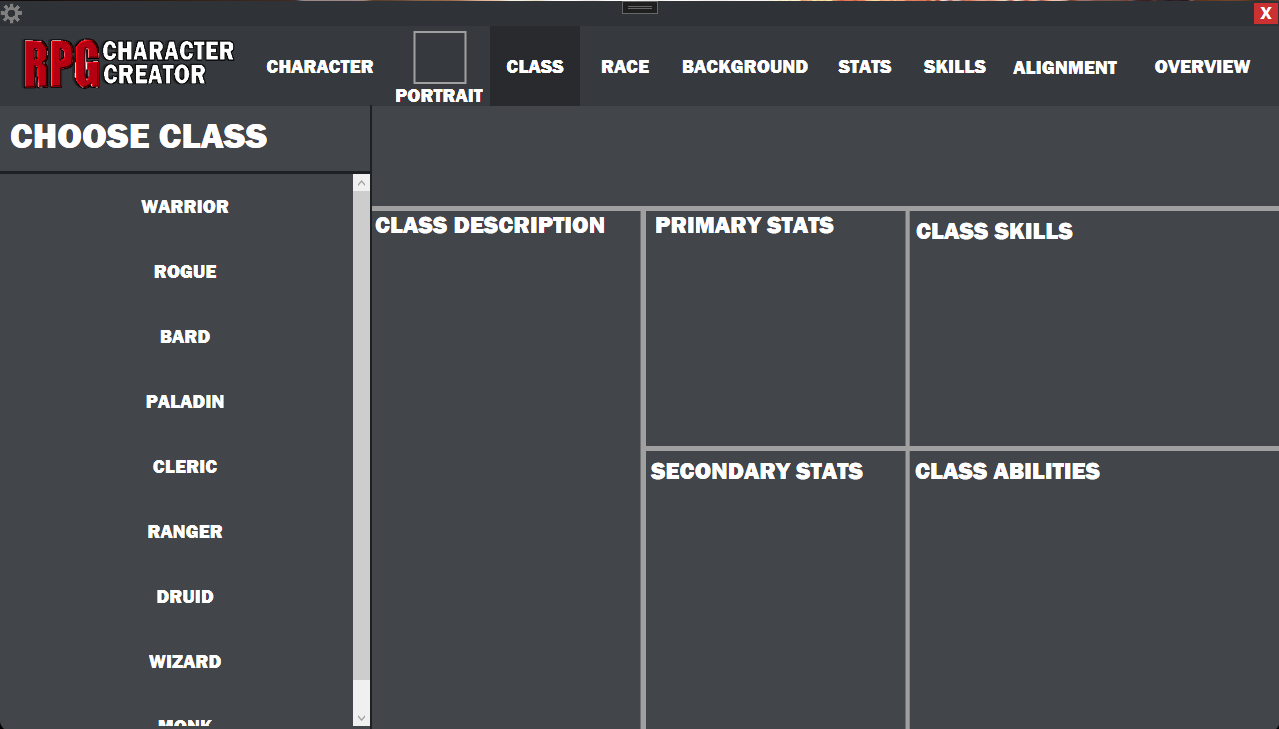
\includegraphics[height=240px, width=426px]{Finished Interface/classScreen.png}
\caption{Class Screen}
\centering
\end{figure}
The user can select their class.
\begin{figure}[H]
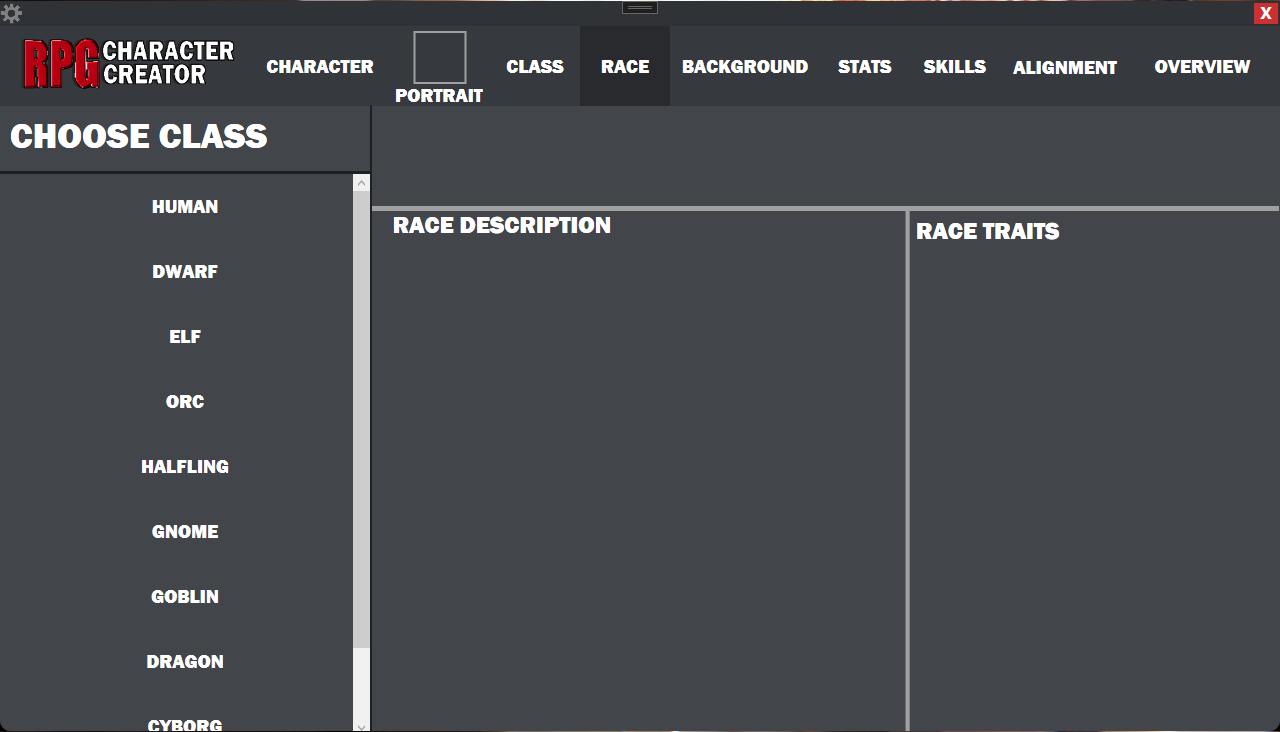
\includegraphics[height=240px, width=426px]{Finished Interface/raceScreen.png}
\caption{Race Screen}
\centering
\end{figure}
The user can select their race.
\begin{figure}[H]
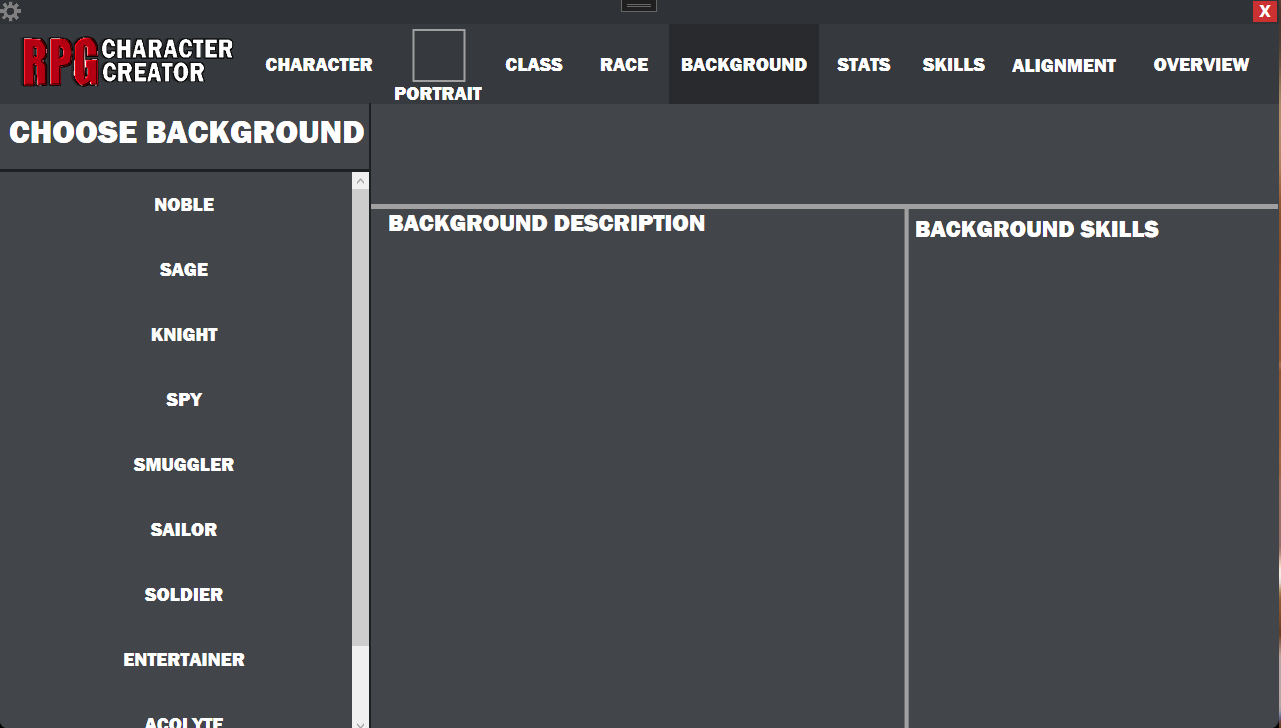
\includegraphics[height=240px, width=426px]{Finished Interface/backgroundScreen.png}
\caption{Background Screen}
\centering
\end{figure}
The user can select their background.
\begin{figure}[H]
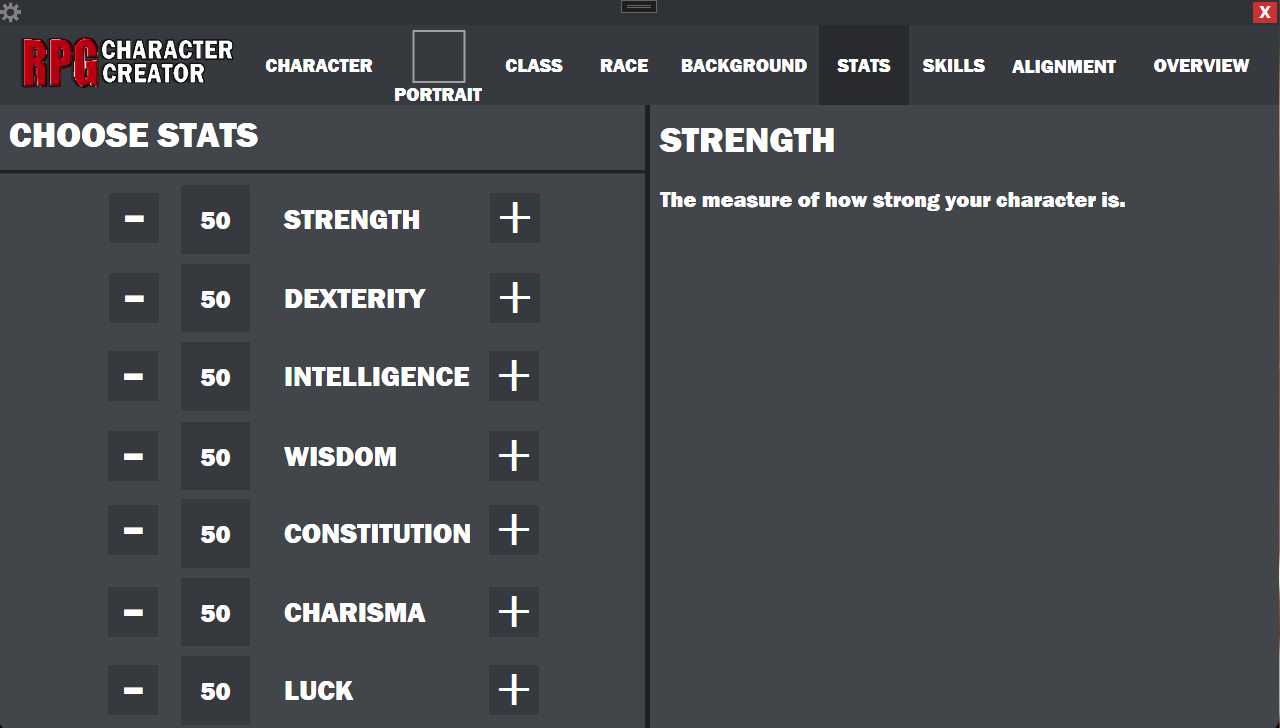
\includegraphics[height=240px, width=426px]{Finished Interface/statsScreen.png}
\caption{Stats Screen}
\centering
\end{figure}
The user can increase or decrease their stats.
\begin{figure}[H]
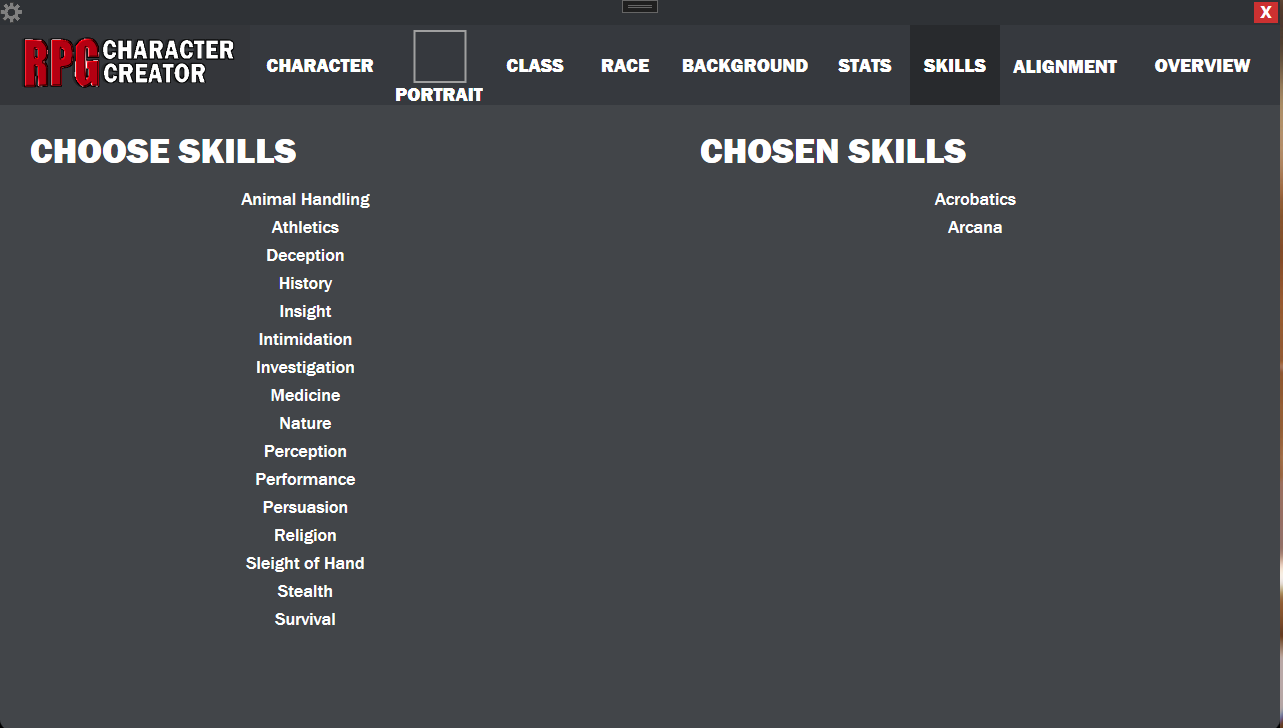
\includegraphics[height=240px, width=426px]{Finished Interface/skillsScreen.png}
\caption{Skills Screen}
\centering
\end{figure}
The skills from background are inherited, and the user can pick from the skills in the left panel.
\begin{figure}[H]
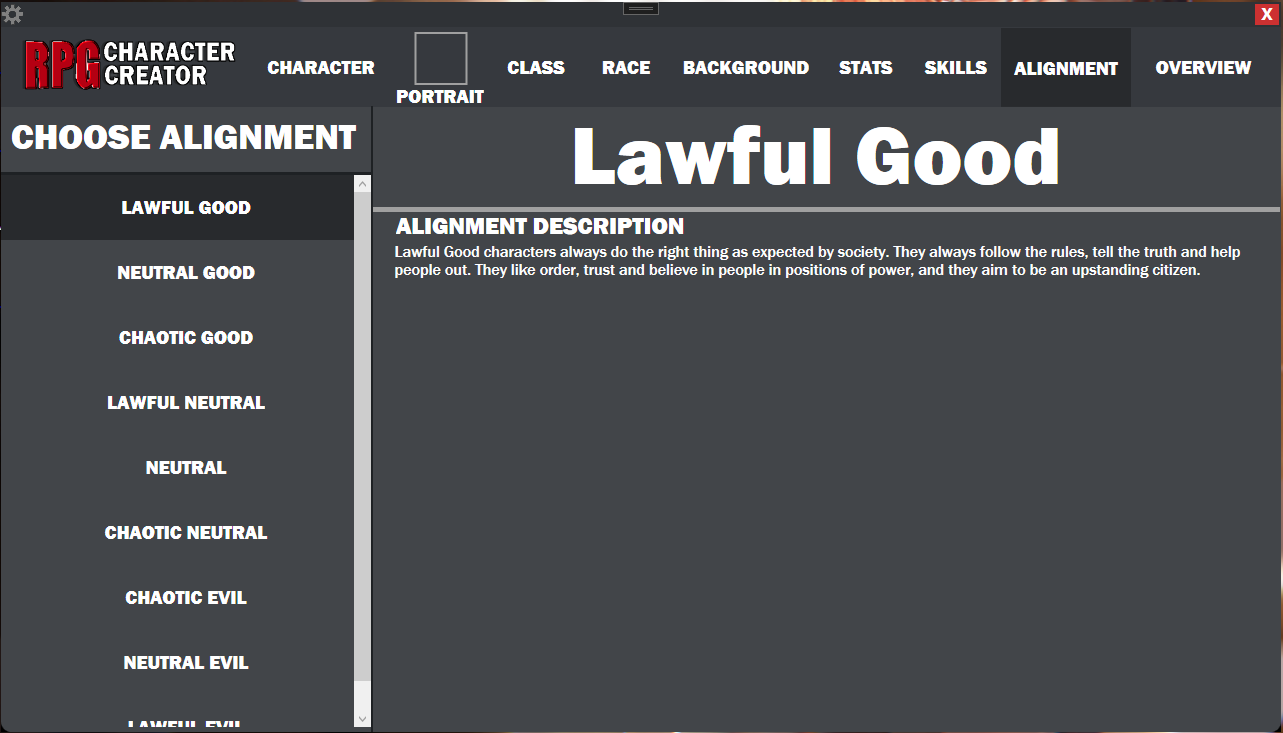
\includegraphics[height=240px, width=426px]{Finished Interface/alignmentScreen.png}
\caption{Alignment Screen}
\centering
\end{figure}
The user can choose their character's alignment.
\begin{figure}[H]
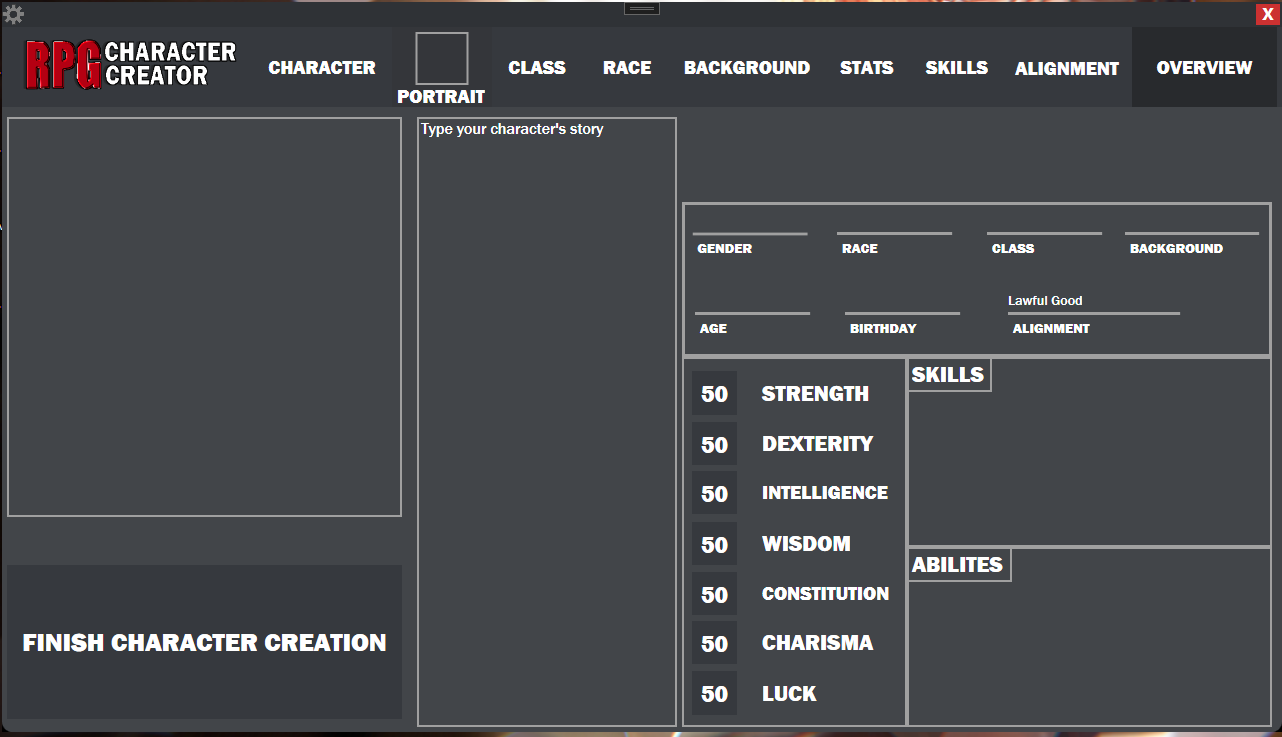
\includegraphics[height=240px, width=426px]{Finished Interface/overviewScreen.png}
\caption{Overview Screen}
\centering
\end{figure}
The user can look over their character and then finish it by pressing the Finish Character Creation Button. This adds the character to the system and they can save it by exiting the program by pressing the x in the top right corner.

\section{Project Timeline}
\textbf{Project Proposal Draft (February 04, 2023)} - First, we brainstormed ideas for a project that would be worth pursuing, and then we drafted a project proposal. This proposal included a project name, an abstract, an introduction, and a scope. Finally, we created a Github repository and uploaded the proposal to it.
\\[10pt]
\textbf{Project Proposal Update (February 28, 2023)} - The update to the project proposal involved identifying the use cases for the project, as well as defining its functional and non-functional requirements. In addition, several interface mockups were created to show our vision for the project.
\\[10pt]
\textbf{GUI Day (March 9th, 2023)}  - Showcased our interface mockups to the class and gathered feedback on potential additions or modifications to our interface mockups.
\\[10pt]
Coding of the actual project began during these two periods beginning with the implementation of a basic UI and building upon it leading up to demo day.
\\[10pt]
\textbf{Demo Day (April 6th, 2023)} - Presented the current status of our project to our classmates and Dr. Ericson.
\\[10pt]
\textbf{Project Update (April 10th, 2023)} - We created a timeline to showcase the progression we have made so far, which involved adding project structure and outlining UML diagrams to project documentation.
\\[10pt]
\textbf{Penultimate Writeup(April 21, 2023)} - We plan to revisit our work and make necessary updates to our documentation to ensure that it is accurate and up-to-date by the specified time.
\\[10pt]
\textbf{Presentation Draft (April 21, 2023)} - We plan on finishing a draft for our presentation slides.
\\[10pt]
\textbf{Final presentation(April 29, 2023)} - We plan on finishing our project and giving our final presentation to the class.
\\[10pt]
\textbf{Final Written Report (April 28, 203)} - We plan on having our final written report that will contain all needed information to show what we have accomplished.

\section{Project Structure}
	First, we needed to determine our target audience. In our case, we decided that this RPG character creator would be geared towards everyone, including both experienced and beginner RPG players. We wanted to make the process as smooth as possible for the user, so we decided on having an easy-to-navigate user interface. We designed the RPG character creator with several sections, including Character which includes the basic character information such as name, age, birthday, and gender. There is also a portrait section where users can choose from pre-selected images or upload their own. The race, background, and alignment section allows users to choose from multiple options, and their information is filled in accordingly. There is also a stats and skills section and an overview page that lets users review their character's details before finalizing the creation process.
	
	In order to stay organized throughout the development stage, we have decided to implement the builder design pattern in our RPG character creator application. By using this pattern, we can easily create complex objects (Characters in our case) by building them step by step. The builder pattern offers the advantage of creating multiple types of objects using the same interface, which will be helpful for our application since users can create a variety of RPG characters.We also implemented the abstract factory design pattern which will be used to create different color themes for the application, easily allowing user to switch between different themes without affecting the functionality or structure of the application.
	
In addition to the design patterns, we have also implemented the Model-View-ViewModel (MVVM) architecture in our RPG character creator application. MVVM helps to cleanly separate the GUI and program logic allowing for better maintainability and testability.

\subsection{UML Outline}
\begin{figure}[ht!]
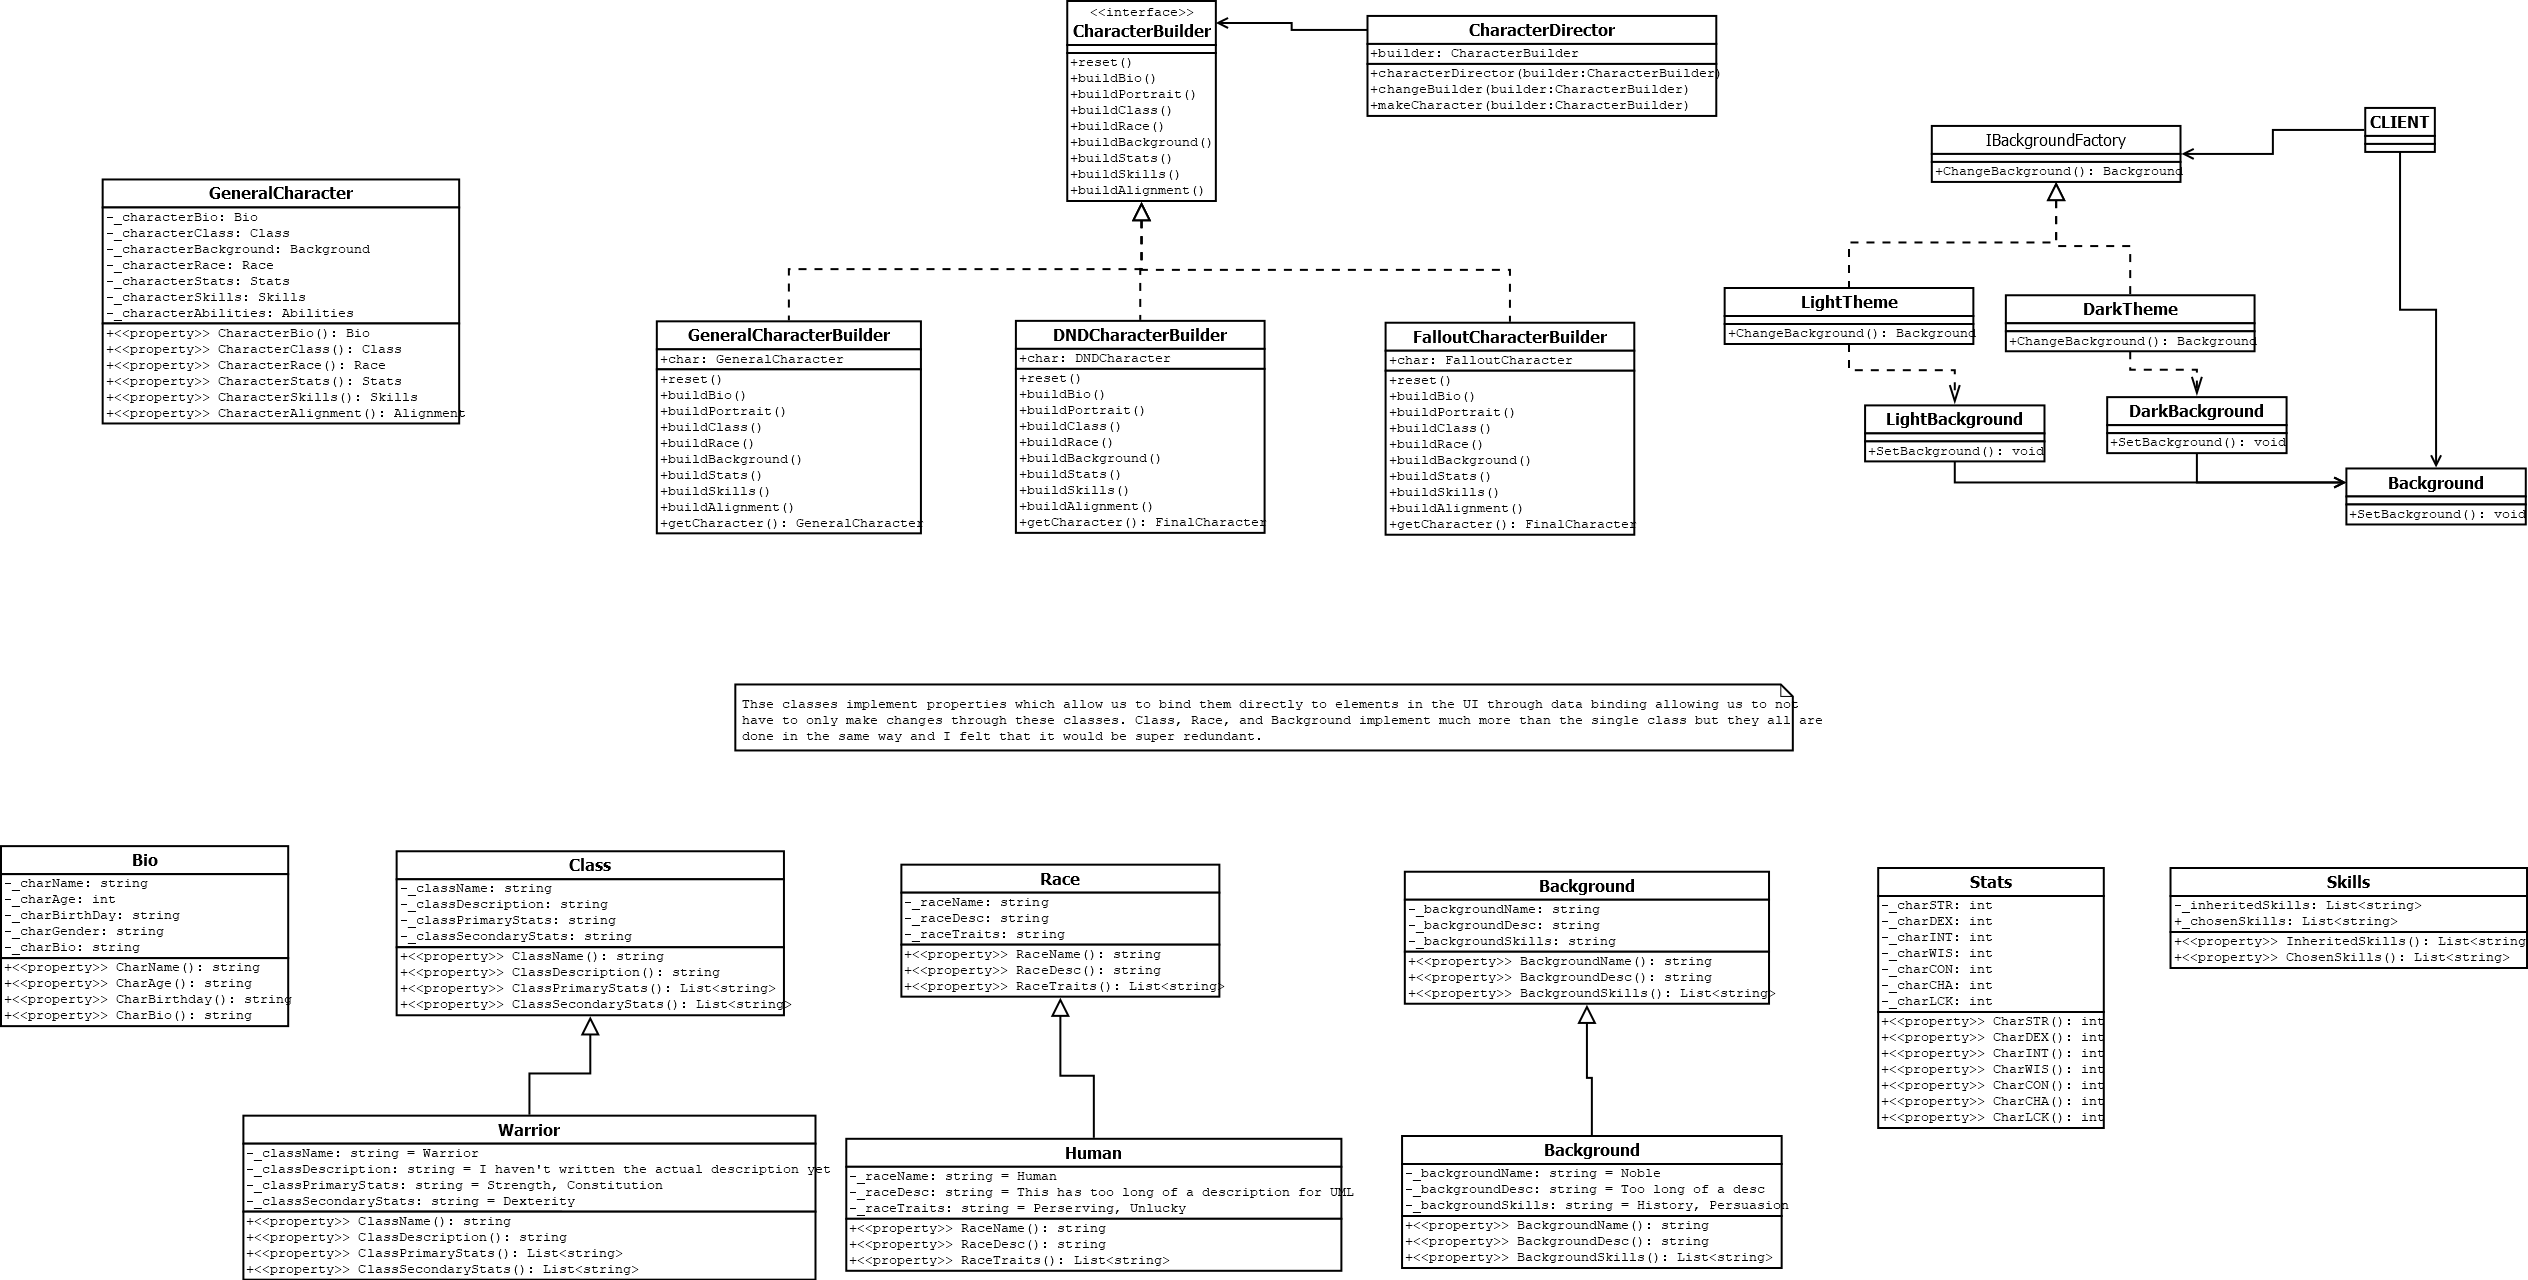
\includegraphics[scale=0.19]{RPGCharacterCreatorUML.png}
\caption{The entire UML for the project}
\label{fullUML}
\end{figure}
\begin{figure}[ht!]
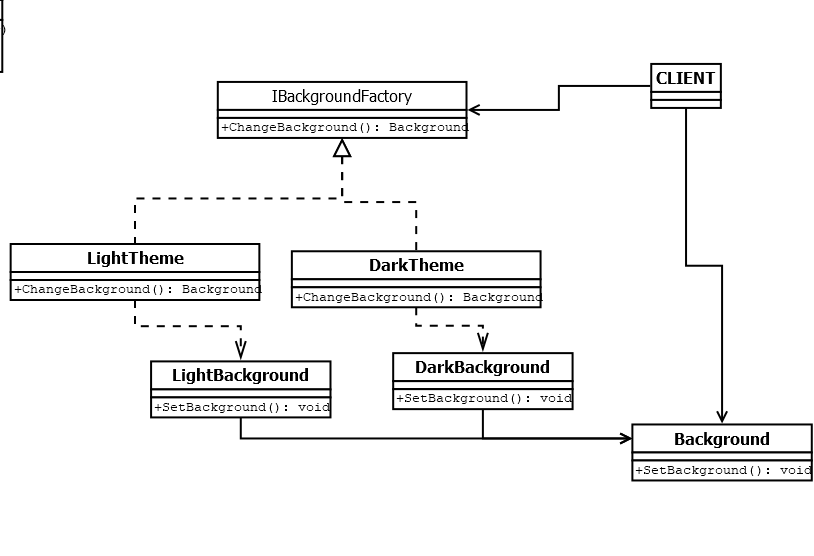
\includegraphics[scale=0.4]{factMethod.png}
\caption{Possible implementation for a factory method that allows for us to easily change the theme of the UI.}
\label{themeFact}
\end{figure}

The following UML is an Factory Design pattern see Figure \ref{themeFact}

The BackgroundFactory is an abstract class that defines a factory method, ‘CreateBackground()’ , which returns a Background object.

The LightTheme and DarkTheme classes are concrete implementations of the BackgroundFactory class. Each class provides a different implementation of the CreateBackground() method, which creates a Background object that has a different color theme.

The Background class is a product of the BackgroundFactory class. It defines a set of properties and methods that allow clients to interact with the background object, such as getting and setting the background color.

Clients of the BackgroundFactory pattern use the factory method to create a Background object without having to know the implementation details of the factory or the product.
\\[10pt]
The following UML is a Builder Design pattern see Figure \ref{charAndBuilder}.

The CharacterBuilder interface specifies the steps for building a character. 

The GeneralCharacterBuilder class implements this interface and is responsible for building the character. 

The CharacterDirector class instructs the GeneralCharacterBuilder on the steps to building a character.
 The GeneralCharacter object is the complex object, and the CharacterBuilder interface defines the steps required to construct it. 

The GeneralCharacterBuilder class implements these steps in its methods.

The CharacterDirector class acts as a director, which looks over  the construction process and can create a specific type of character by using a specific implementation of the CharacterBuilder interface.



\begin{figure}[ht!]
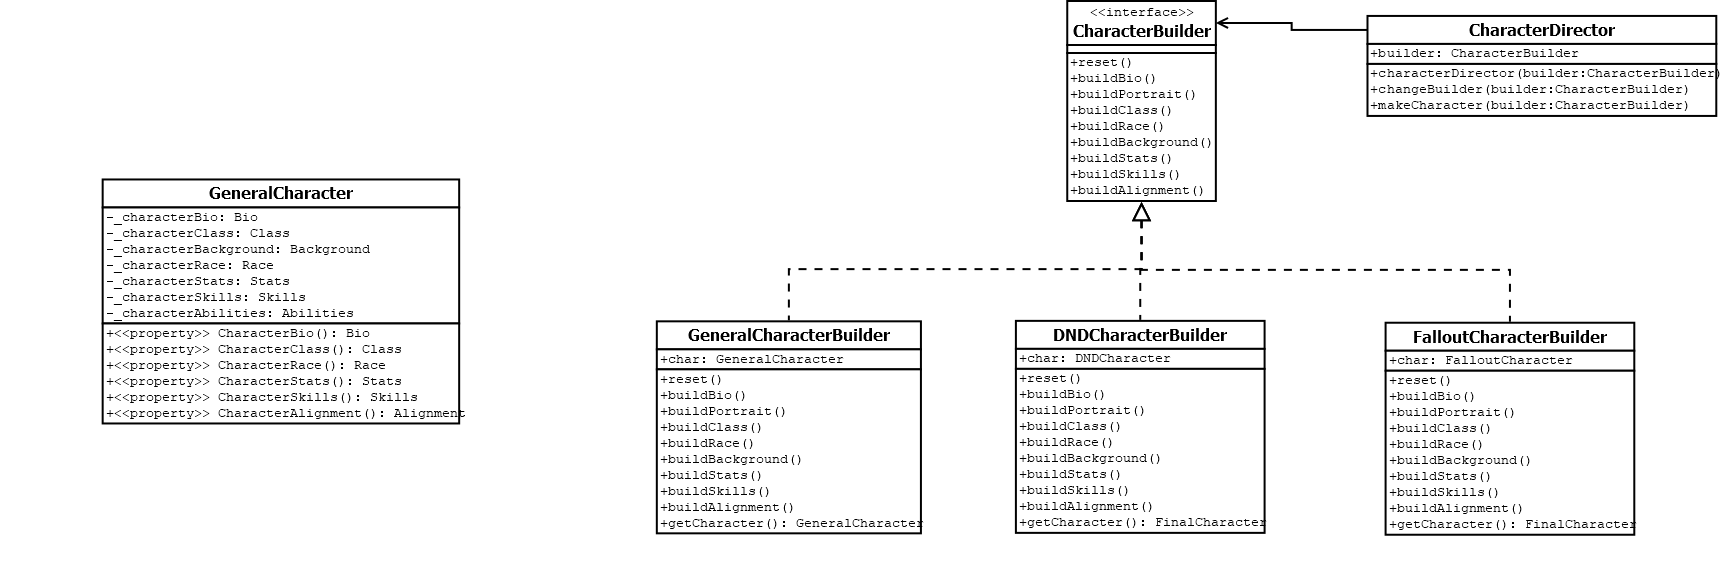
\includegraphics[scale=0.39]{builderAndChar.png}
\caption{The Builder of the project, the generalCharacterBuilder creates a general character and through the director builds a generalCharacter with each of its variables being assigned through the builder.}
\label{charAndBuilder}
\end{figure}

\begin{figure}[ht!]
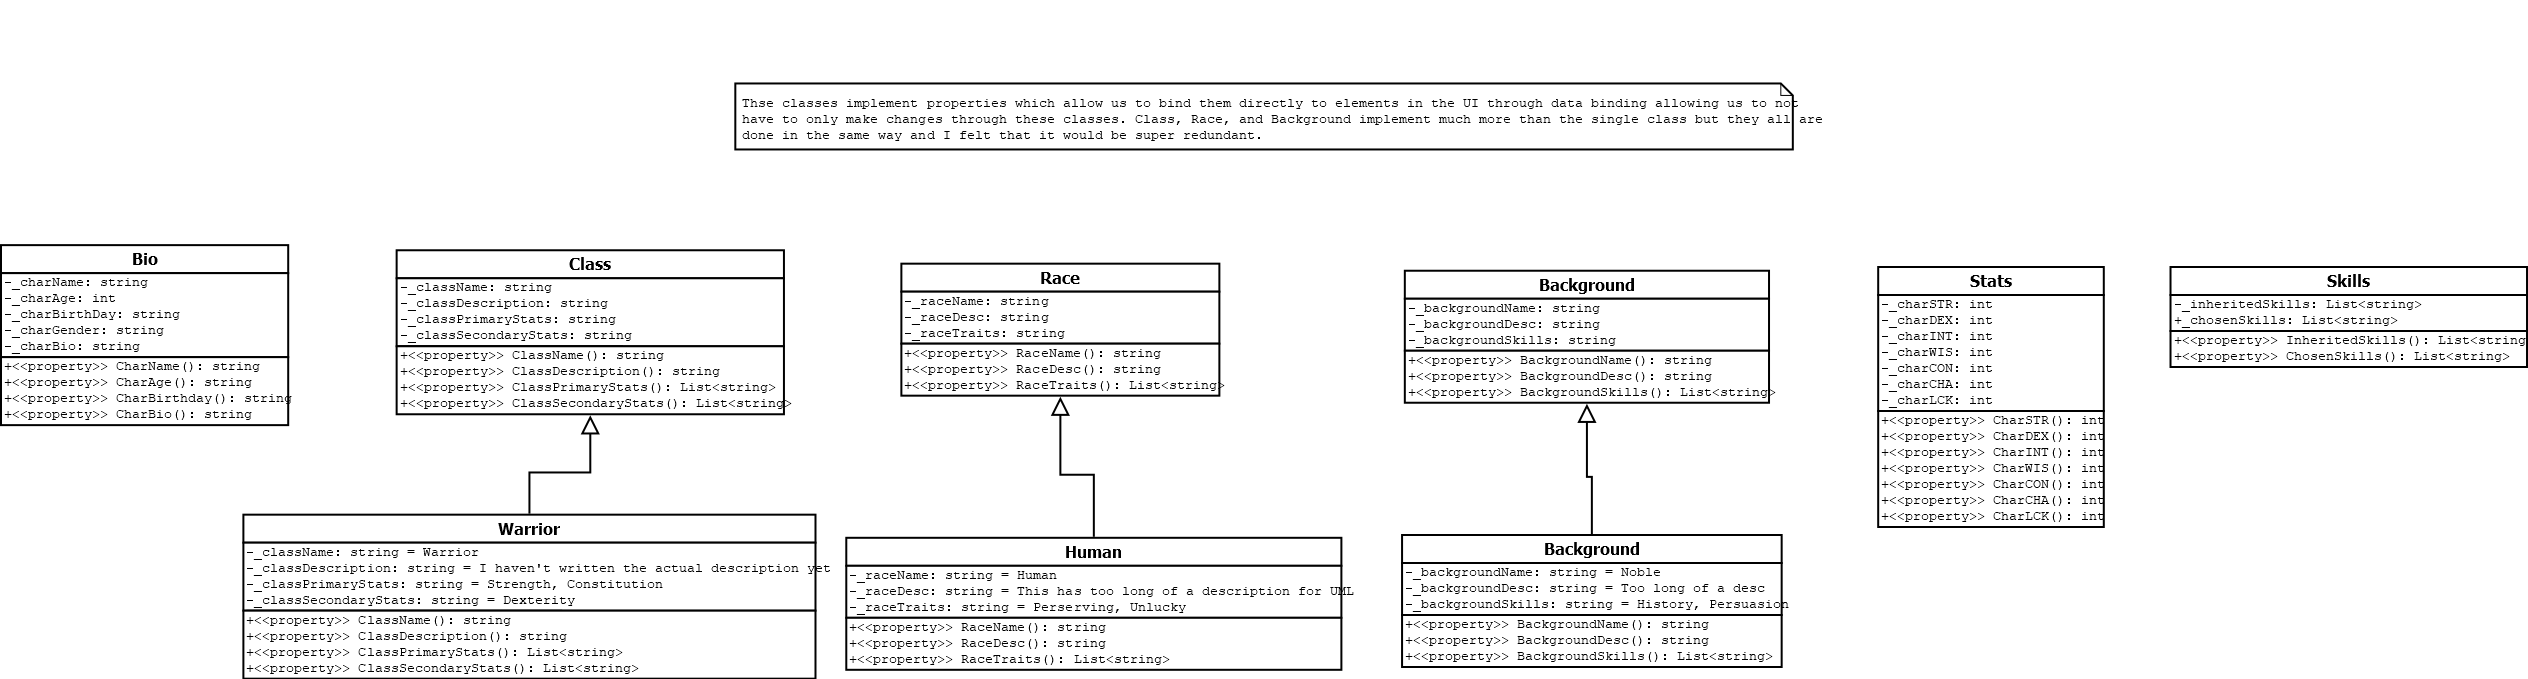
\includegraphics[scale=0.28]{CharStuff.png}
\caption{The generalCharacter is made of these classes, these classes store information and allow for us to easily update the UI through the use of data binding and properties.}
\label{charStuff}
\end{figure}




\subsection{Design Patterns Used}
We used the builder design pattern which allows us to build a character all in one step. We first gather all the information need to create a character then call the builder through the director which creates a character with all the information that we need for the character. It can also create empty characters which the user can go back and edit.
To implement different themes for the UI we implemented a factory method which allows us to easily create different themes. All of the UI elements are bound to different variables and the factory method assigns these variables different color values. This allows for us to add many different themes and if we need to, edit already create themes.

\section{Results}
Outside of the stretch goals, I think that the project ended up where we wanted it to when we first came up with the idea. Right now its scope is somewhat limited but for the most part it covers the most commonly used characteristics that define traditional RPG characters. The framework is there for being able to implement a means of creating custom classes, races, backgrounds, etc. which would greatly increase the applicability of the application. While it is done in the sense that it works like we first planned it to, there is still parts of the project that need some "love" added to them. Quality of life(QoL) features such search bars, sorting, tool tips are definitely missing from the project. Overall, we are happy with what we were able to accomplish with one of first major projects.
\subsection{Future Work}
In the future, like mentioned in the results section, there is a need for some QoL features and some love to go towards the more neglected parts of the project. While the implementation of different RPG systems would require a major rework of how the current UI is implemented, adding a DM mode would not. This DM mode would allow for the user them self to cover any areas of character creation that we might of missed allowing for them to get their character exactly how they want them. 



\begin{thebibliography}{1}

\bibitem{IEEEhowto:kopka}
H.~Kopka and P.~W. Daly, \emph{A Guide to \LaTeX}, 3rd~ed.\hskip 1em plus
  0.5em minus 0.4em\relax Harlow, England: Addison-Wesley, 1999.

\end{thebibliography}



\begin{IEEEbiography}{Michael Shell}
Biography text here.
\end{IEEEbiography}

% if you will not have a photo at all:
\begin{IEEEbiographynophoto}{John Doe}
Biography text here.
\end{IEEEbiographynophoto}

% insert where needed to balance the two columns on the last page with
% biographies
%\newpage

\begin{IEEEbiographynophoto}{Jane Doe}
Biography text here.
\end{IEEEbiographynophoto}





% that's all folks
\end{document}


